\title{Лекция 17\\Представление в базе знаний временных сущностей}
\author[]{Шункевич Д.В.}
\institute[]{Белорусский государственный университет информатики и радиоэлектроники}

\begin{frame}
	\titlepage
\end{frame}

\begin{frame}{\\Содержание лекции}
	\topline
	\justifying
	Понятие временной сущности, классификация. Описания взаимосвязи событий. Причинно-следственные связи, их представление в базе знаний. Понятие процесса, ситуации, события. Темпоральные отношения, их представление в базе знаний.
\end{frame}

\begin{frame}{\\Понятие временной сущности}
	\topline
	\justifying
	\scnheader{временная сущность}
	\scnidtf{темпоральная сущность}
	\scnidtf{нестационарная сущность}
	\scnidtf{сущность, имеющая и/или начало, и/или конец своего существования}
	\scnidtf{сущность, обладающая темпоральными характеристиками (длительностью, начальным моментом, конечным моментом и т.д.)}
	\begin{scnrelfromset}{разбиение}
		\scnitem{прошлая сущность}
		\scnitem{настоящая сущность}
		\scnitem{будущая сущность}
	\end{scnrelfromset}
\end{frame}

\begin{frame}{\\Понятие временной сущности}
	\topline
	\justifying
	\scnheader{временная сущность}
	\begin{scnrelfromset}{разбиение}
		\scnitem{временная связь}
		\scnitem{темпоральная (временная) структура}
		\begin{scnindent}
			\scnidtf{структура, содержащая хотя бы одну временную сущность}
		\end{scnindent}
		\scnitem{материальная сущность}
	\end{scnrelfromset}
\end{frame}

\begin{frame}{\\Классификация временных сущностей}
	\topline
	\justifying
	\scnheader{временная сущность}
	\begin{scnrelfromset}{разбиение}
		\scnitem{непрерывная временная сущность}
			\begin{scnindent}
			\begin{scnrelfromset}{разбиение}
				\scnitem{точечная временная сущность}
						\begin{scnindent}
						\scnidtf{атомарная (мгновенная) временная сущность}
						\end{scnindent}
				\scnitem{длительная непрерывная временная сущность}
			\end{scnrelfromset}
			\end{scnindent}
		\scnitem{дискретная временная сущность}
				\begin{scnindent}
				\scnidtf{временная сущность, которая может быть декомпозирована на последовательность точечных временных сущностей}
				\end{scnindent}
		\scnitem{прерывистая временная сущность}
			\begin{scnindent}
			\scnidtf{временная сущность с прерываниями}
			\end{scnindent}
	\end{scnrelfromset}
\end{frame}

\begin{frame}{\\Временная связь} %?
	\topline
	\justifying
	Каждая временная связь представляет собой связку, принадлежащую множеству временных сущностей.\\
	Понятие временной связи не следует путать с понятием темпоральной связи, которая сама является постоянной
	сущностью, описывающей то, как связаны во времени некоторые временные сущности.
\end{frame}

\begin{frame}{\\Понятие процесса, ситуации, события}
	\topline
	\justifying
	\scnheader{темпоральная структура}
	\begin{scnrelfromset}{разбиение}
		\scnitem{ситуация}
		\begin{scnindent}
			\scnidtf{статическая временная структура}
		\end{scnindent}
		\scnitem{процесс}
		\begin{scnindent}
			\scnidtf{динамическая временная структура}
		\end{scnindent}
	\end{scnrelfromset}
\end{frame}

\begin{frame}{\\Ситуация}
	\topline
	\justifying
	Под ситуацией понимается структура, содержащая, по крайней мере, один элемент, который является временной
	сущностью. Наличие в рамках ситуации нескольких временных сущностей говорит о том, что существует момент	времени (в прошлом, настоящем или будущем), в который все они существуют одновременно.
	\scnheader{ситуация}
	\scnidtf{временная структура}
	\scnidtf{состояние некоторой динамической системы, описываемое с некоторой степенью детализации (подробности)}
\end{frame}

\begin{frame}{\\Процесс}
	\topline
	\justifying
	
	\vspace{10mm}
	Процесс задается возникновением или исчезновением связей, связывающих заданную временную сущность с другими сущностями.\\
	Процессу можно поставить в соответствие его \textbf{\textit{начальную ситуацию*}} и \textbf{\textit{конечную ситуацию*}}, то есть указать ситуации, переход между которыми осуществляется в ходе процесса.
	\scnheader{процесс}
	\scnidtf{динамическая структура}
	\scnidtf{процесс преобразования некоторой временной сущности из одного состояния в другое}
	\begin{scnrelfromset}{разбиение}
		\scnitem{точечный (мгновенный) процесс}
		\scnitem{элементарный (атомарный) процесс}
	\end{scnrelfromset}
\end{frame}

\begin{frame}{\\Событие}
	\topline
	\justifying
	\scnheader{событие}
	\scnidtf{граничная точка временной сущности}
	\scnidtf{точечная временная сущность, являющаяся началом и/или завершением какой-либо временной сущности
	(например, процесса)}
\end{frame}

\begin{frame}{\\Событие}
	\topline
	\justifying
	\vspace{10mm}
	\begin{SCn}
		\begin{figure}[H]
			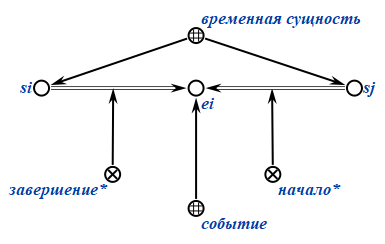
\includegraphics[scale=0.8]{./figures/sd_temp_entities/event.png}
		\end{figure}
	\end{SCn}
\end{frame}

\begin{frame}{\\\textbf{\textit{событие*}}}
	\topline
	\justifying
	\scnheader{событие*}
	\scniselement{бинарное отношение}
	\scntext{пояснение}{Связки отношения \textit{событие*} связывают знак процесса и ориентированную пару, первым компонентом которой	является знак \textit{начальной ситуации*} данного процесса, вторым компонентом -- знак \textit{конечной ситуации*} данного процесса}
\end{frame}

\begin{frame}{\\\textbf{\textit{событие*}}}
	\topline
	\justifying
	\vspace{10mm}
	\begin{SCn}
		\begin{figure}[H]
			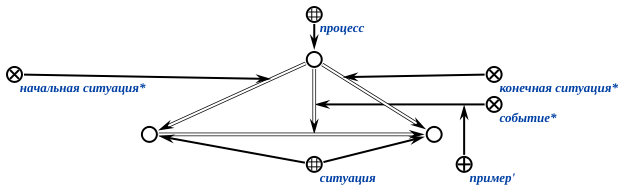
\includegraphics[scale=0.7]{./figures/sd_temp_entities/nrel_event.png}
		\end{figure}
	\end{SCn}
\end{frame}

\begin{frame}{\\Пример ситуации}
	\topline
	\justifying
	\vspace{10mm}
	\begin{SCn}
		\begin{figure}[H]
			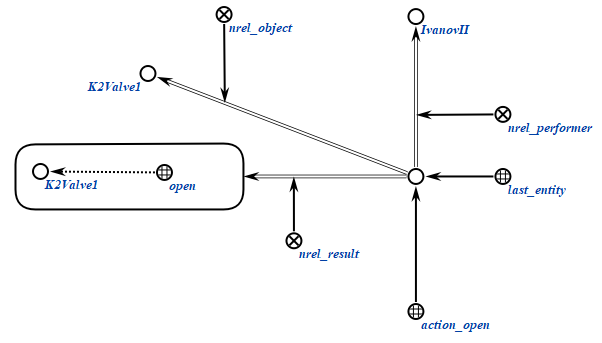
\includegraphics[scale=0.7]{./figures/sd_temp_entities/valve_opening.png}
		\end{figure}
	\end{SCn}
\end{frame}

\begin{frame}{\\Пример процесса}
\topline
\justifying
\vspace{10mm}
\begin{SCn}
	\begin{figure}[H]
		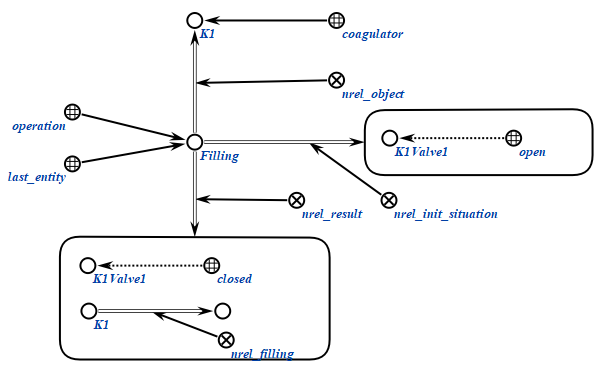
\includegraphics[scale=0.7]{./figures/sd_temp_entities/process_description.png}
	\end{figure}
\end{SCn}
\end{frame}

\begin{frame}{Темпоральные отношения}
	\topline
	\justifying
	\scnheader{темпоральное отношение}
	\scnrelto{семейство подмножеств}{темпоральная связь}
	\scnhaselement{темпоральное включение*}
	\scnhaselement{темпоральное объединение*}
	\scnhaselement{темпоральная декомпозиция*}
	\scnhaselement{темпоральная последовательность*}
	\begin{scnindent}
		\begin{scnrelfromset}{разбиение}
			\scnitem{темпоральная смежность*}
			\scnitem{темпоральная последовательность с промежутком*}
			\scnitem{темпоральная последовательность с пересечением*}
		\end{scnrelfromset}
	\end{scnindent}
\end{frame}

\begin{frame}{\\Темпоральная декомпозиция}
	\topline
	\justifying
	\vspace{10mm}
	\begin{SCn}
		\begin{figure}[H]
			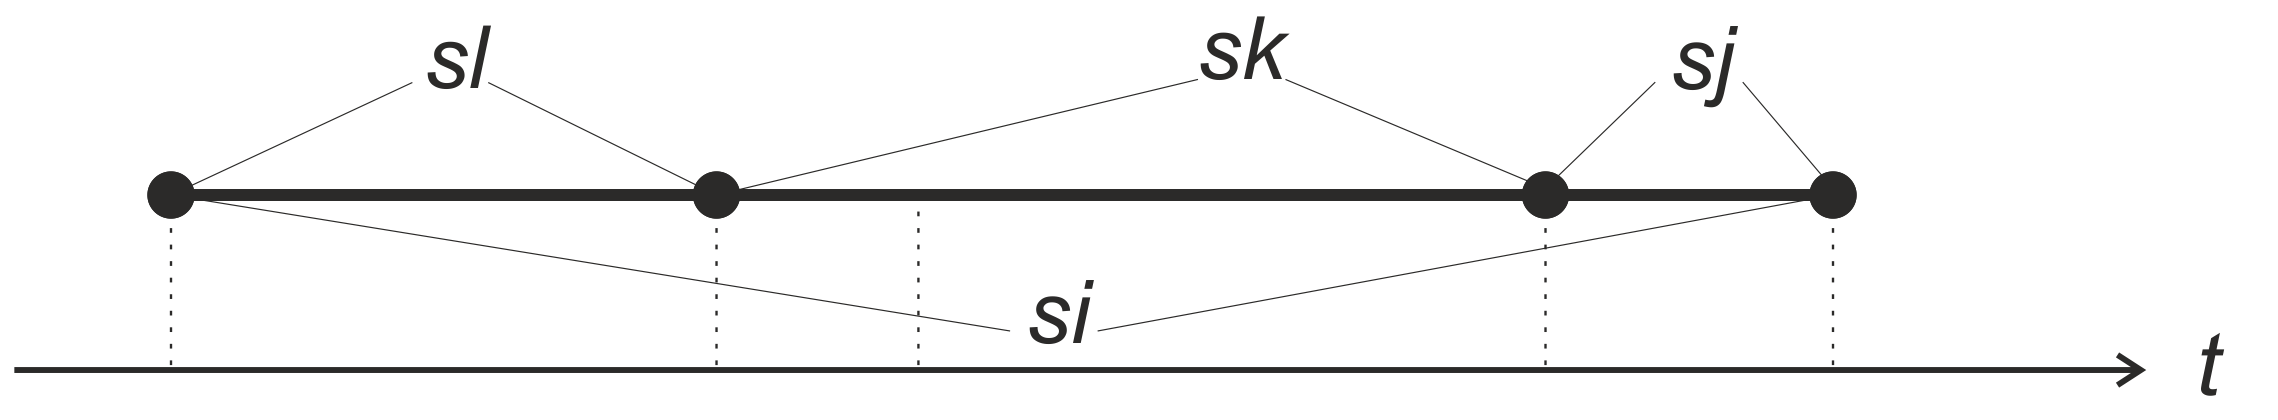
\includegraphics[scale=0.6]{./figures/sd_temp_entities/img_temporal_decomposition.png}
		\end{figure}
	\end{SCn}
\end{frame}

\begin{frame}{\\Темпоральное объединение}
	\topline
	\justifying
	\vspace{10mm}
	\begin{SCn}
		\begin{figure}[H]
			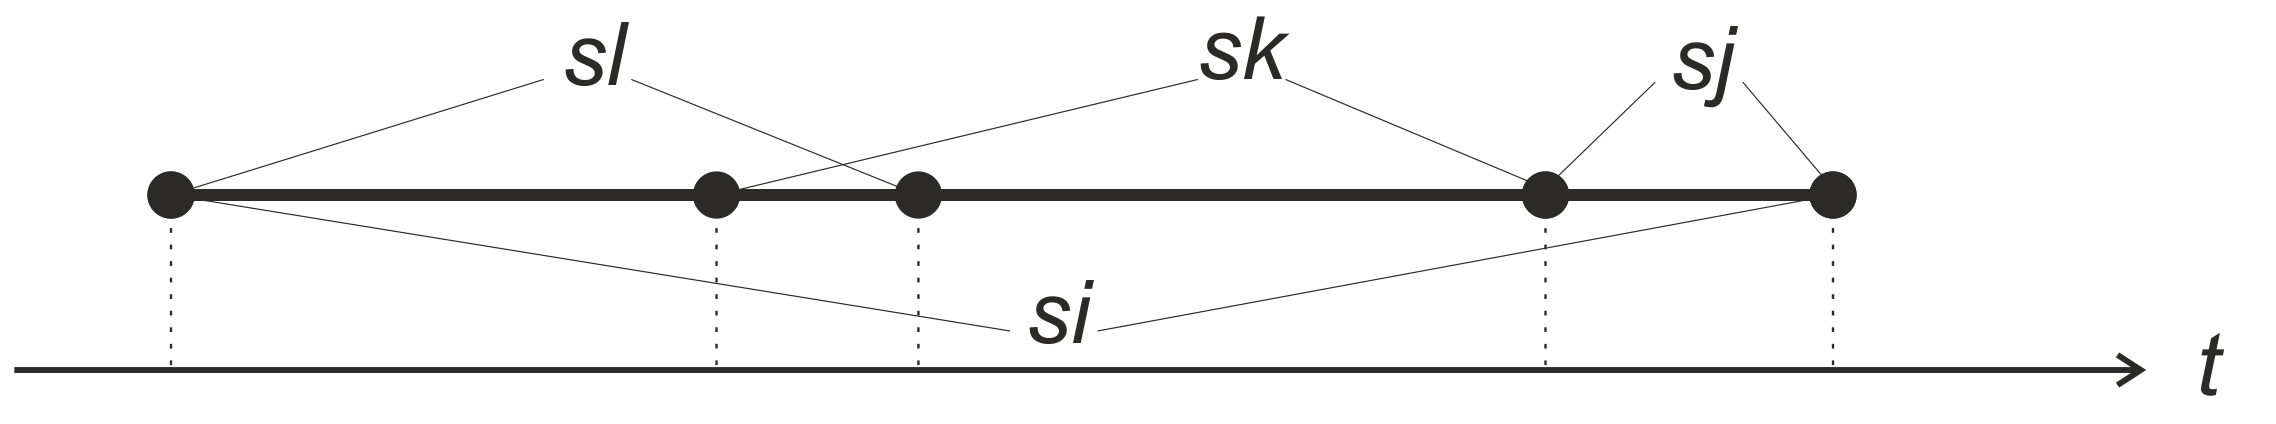
\includegraphics[scale=0.6]{./figures/sd_temp_entities/img_temporal_union.png}
		\end{figure}
	\end{SCn}
\end{frame}

\begin{frame}{\\Темпоральное объединение}
	\topline
	\justifying
	\vspace{10mm}
	\begin{SCn}
		\begin{figure}[H]
			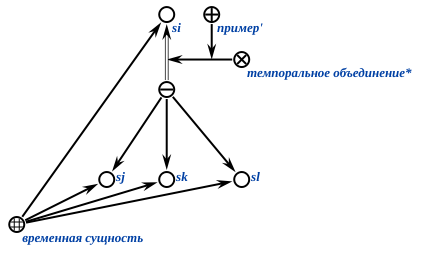
\includegraphics[scale=0.6]{./figures/sd_temp_entities/temporal_union.png}
		\end{figure}
	\end{SCn}
\end{frame}

\begin{frame}{Темпоральное включение}
	\topline
	\justifying
	\vspace{10mm}
	\scnheader{темпоральное включение*}
	\scntext{пояснение}{Связки отношения \textit{темпоральное включение*} связывают две временные сущности, период существования одной из которых полностью включается в период существования второй. Первым компонентом каждой связки отношения \textit{темпоральное включение*} является знак временной сущности, длительность существования которой больше.}
	\scnsuperset{темпоральная часть*}
	\scnsuperset{темпоральное включение без совпадения начальных и конечных моментов*}
	\scnsuperset{темпоральное совпадение*}
	\scnsuperset{темпоральное включение с совпадением начальных моментов*}
	\scnsuperset{темпоральное включение с совпадением конечных моментов*}
\end{frame}

\begin{frame}{\\Темпоральная часть и включение, совпадение}
	\topline
	\justifying
	Связки отношения \textbf{темпоральная часть*} связывают две временные сущности, одна из которых является частью	другой, например, действие и одно из его поддействий. Соответственно, период существования одной из этих сущностей всегда будет включаться в период существования другой (большей).\\
	Более общее отношение -- \textbf{темпоральное включение*}, связки которого могут связывать любые временные сущности.
	\scnheader{темпоральное совпадение*}
	\scnidtf{совпадение начала и завершения*}
\end{frame}

\begin{frame}{\\Темпоральная часть}
	\topline
	\justifying
	\vspace{10mm}
	\begin{SCn}
		\begin{figure}[H]
			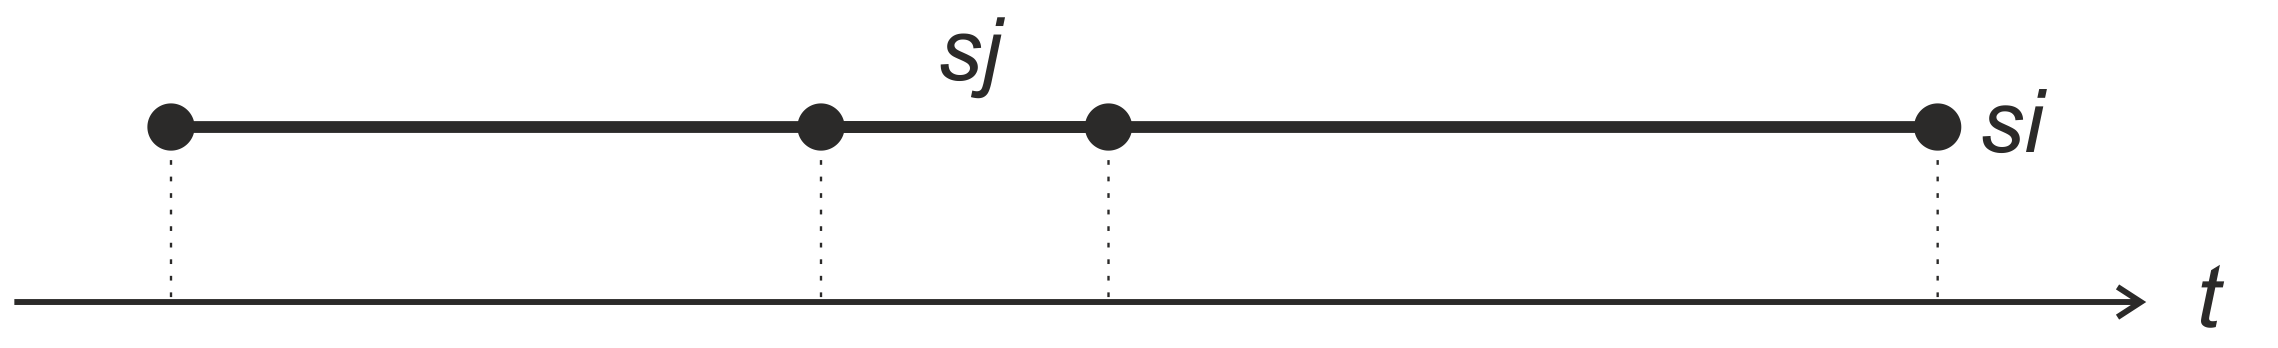
\includegraphics[scale=0.6]{./figures/sd_temp_entities/img_temporal_part.png}
		\end{figure}
	\end{SCn}
\end{frame}

\begin{frame}{\\Темпоральное включение (строгое)}
	\topline
	\justifying
	\vspace{10mm}
	\begin{SCn}
		\begin{figure}[H]
			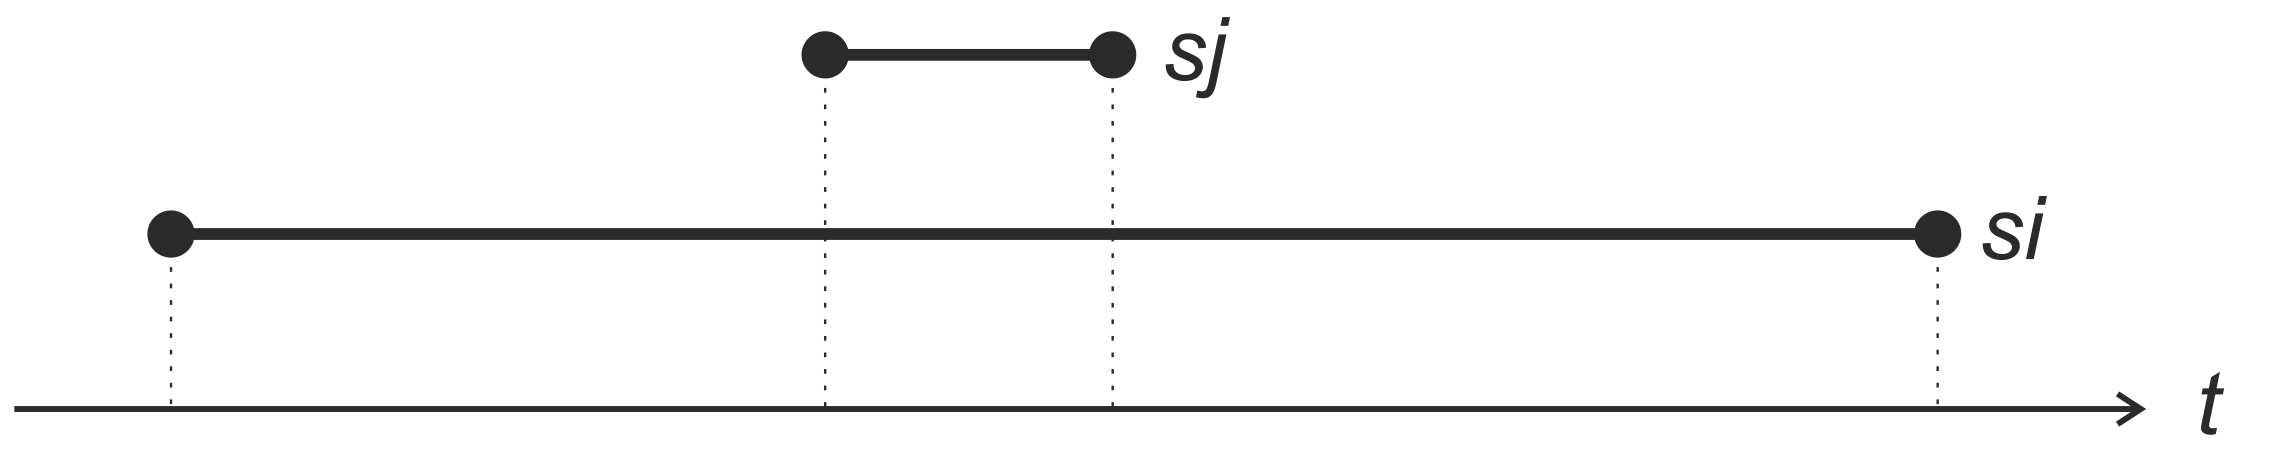
\includegraphics[scale=0.6]{./figures/sd_temp_entities/img_strict_temporal_inclusion.png}
		\end{figure}
	\end{SCn}
\end{frame}

\begin{frame}{Темпоральное включение (совпадение начал)}
	\topline
	\justifying
	\vspace{10mm}
	\begin{SCn}
		\begin{figure}[H]
			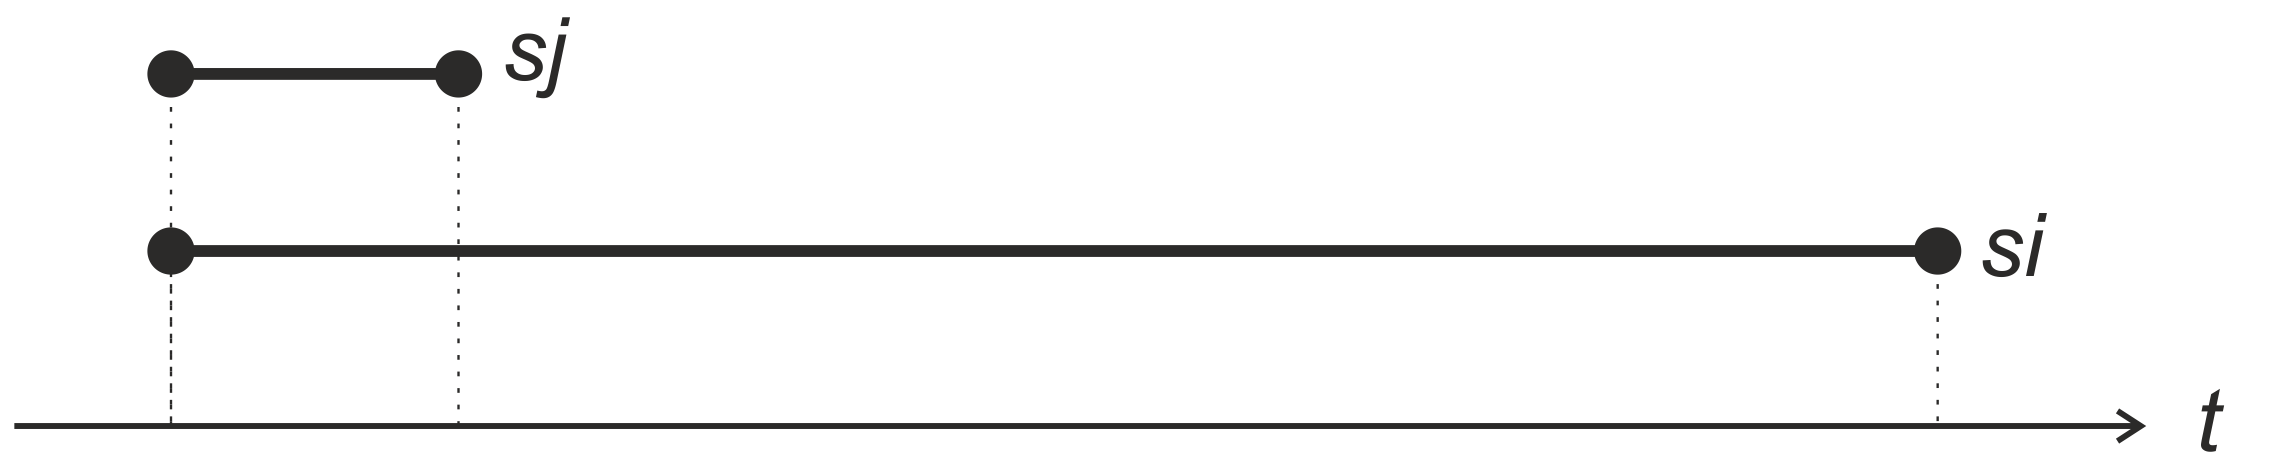
\includegraphics[scale=0.6]{./figures/sd_temp_entities/img_temporal_include_with_match_start_points.png}
		\end{figure}
	\end{SCn}
\end{frame}

\begin{frame}{Темпоральное включение (совпадение завершений)}
	\topline
	\justifying
	\vspace{10mm}
	\begin{SCn}
		\begin{figure}[H]
			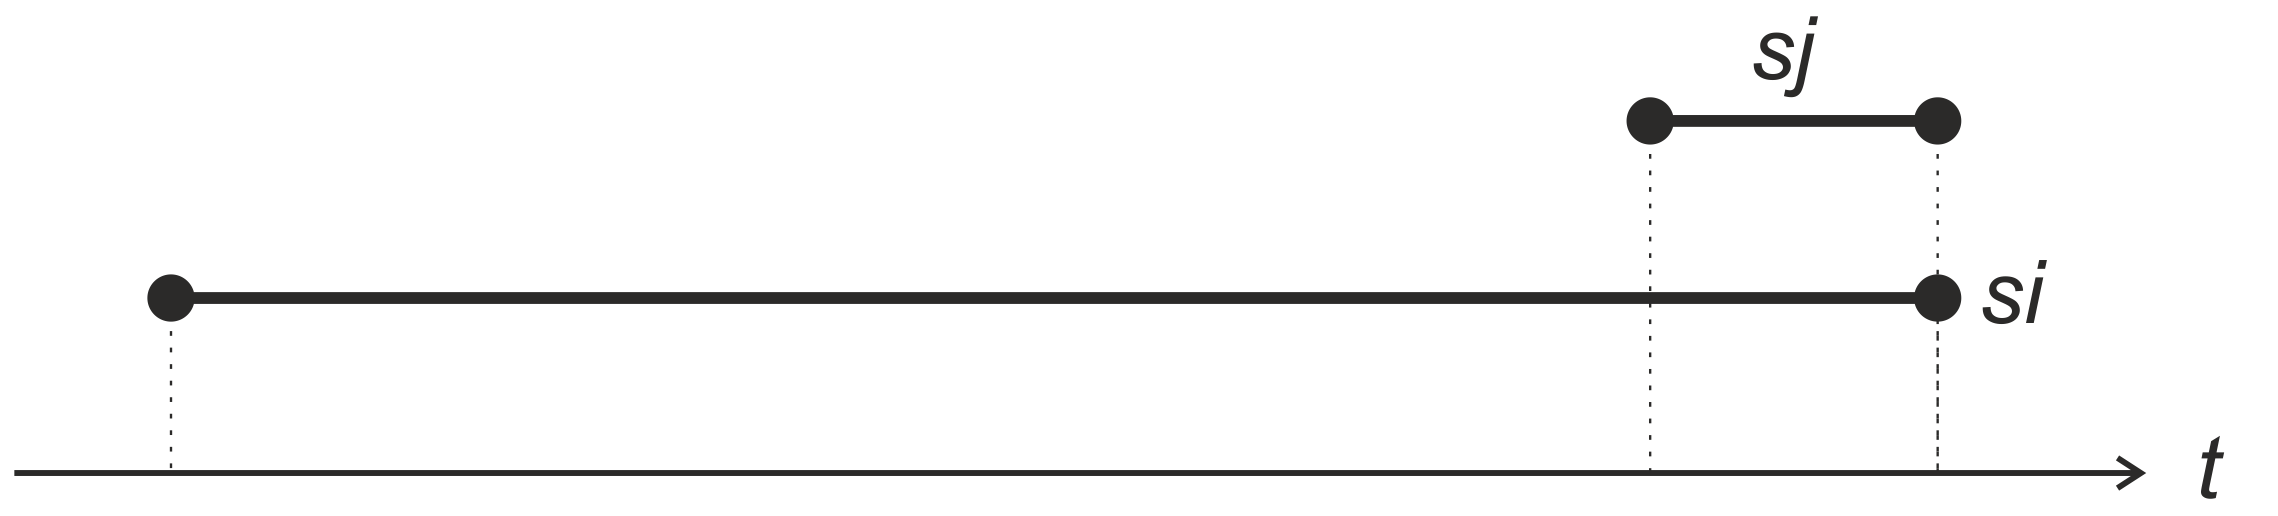
\includegraphics[scale=0.6]{./figures/sd_temp_entities/img_temporal_include_with_terminal_point_match.png}
		\end{figure}
	\end{SCn}
\end{frame}

\begin{frame}{\\Темпоральная смежность}
	\topline
	\justifying
	\scnheader{темпоральная смежность*}
	\scnidtf{темпоральная последовательность без промежутка*}
	\scnidtf{сразу после*}
	\scnheader{темпоральная последовательность с пересечением*}
	\scnheader{темпоральная последовательность с промежутком*}
	\scnidtf{не сразу после*}
\end{frame}

\begin{frame}{\\Темпоральная смежность}
	\topline
	\justifying
	\vspace{10mm}
	\begin{SCn}
		\begin{figure}[H]
			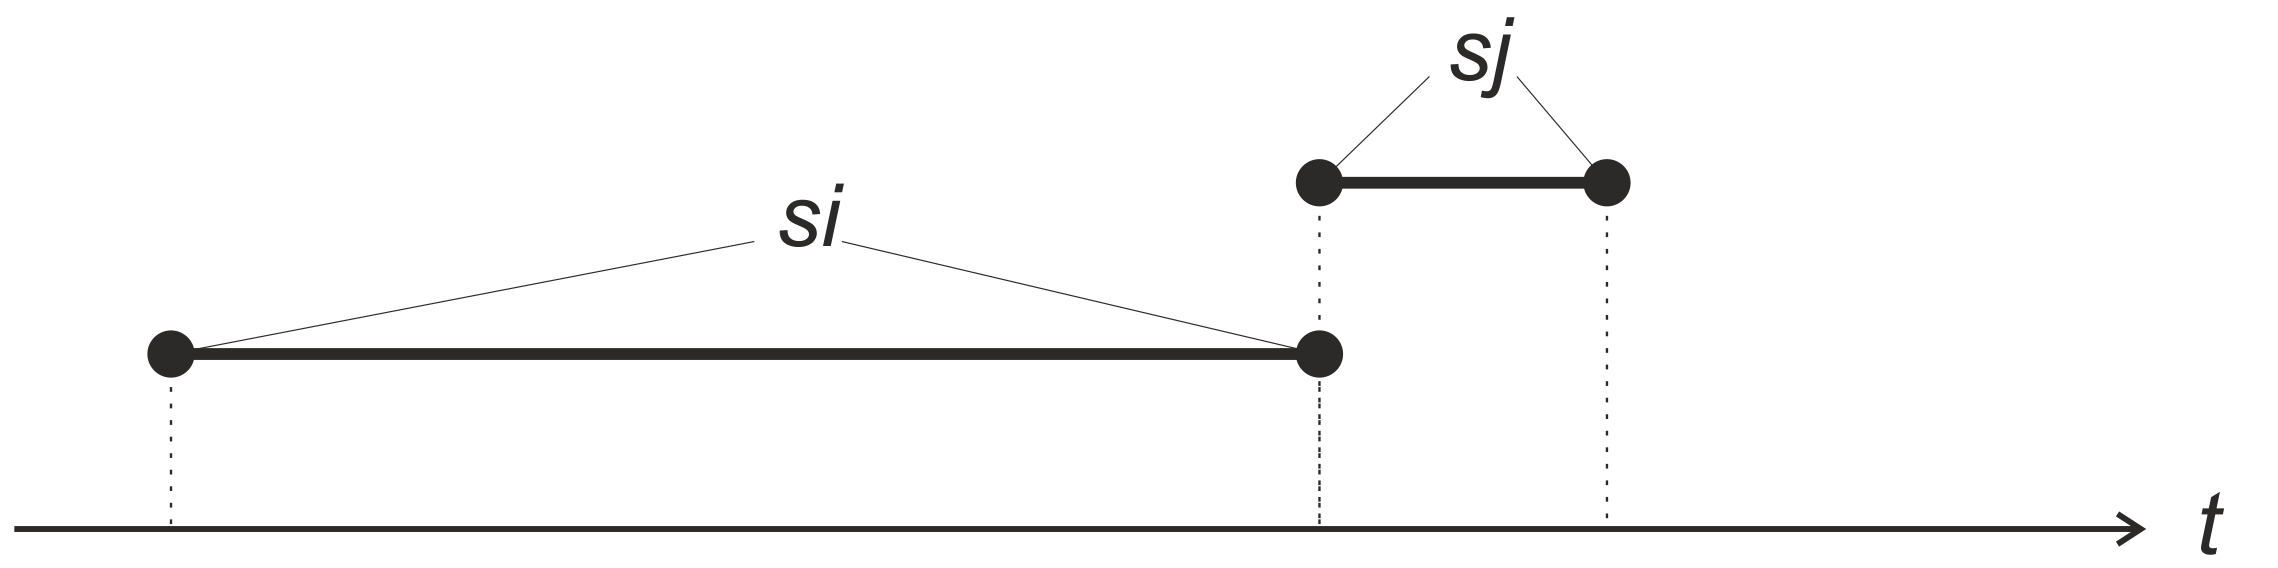
\includegraphics[scale=0.6]{./figures/sd_temp_entities/img_temporal_adjacency.png}
		\end{figure}
	\end{SCn}
\end{frame}

\begin{frame}{Темпоральная последовательность с пересечением}
	\topline
	\justifying
	\vspace{10mm}
	\begin{SCn}
		\begin{figure}[H]
			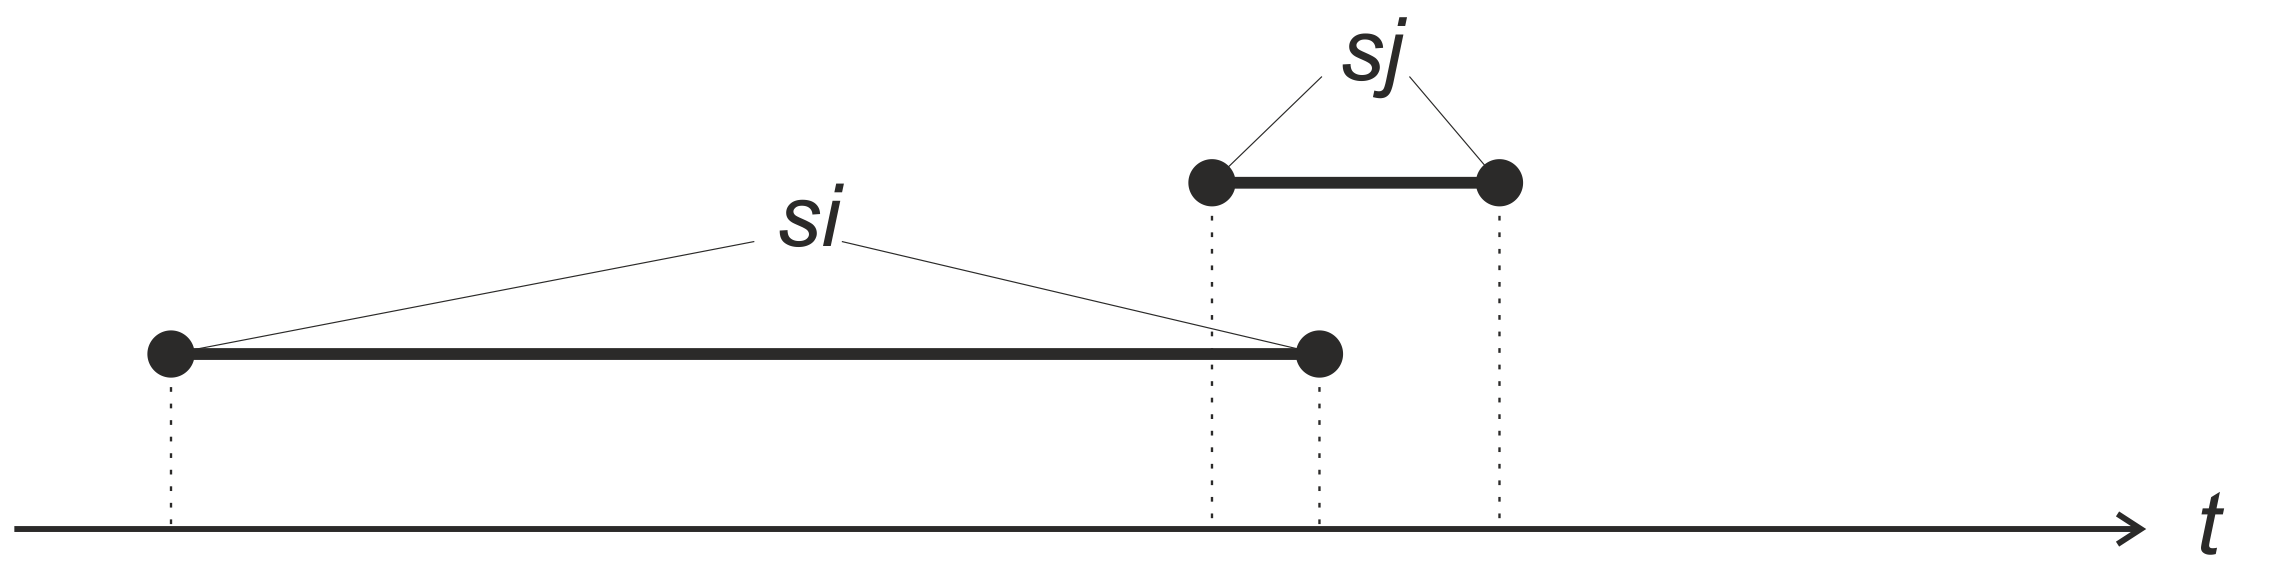
\includegraphics[scale=0.6]{./figures/sd_temp_entities/img_temporal_cross_sequence.png}
		\end{figure}
	\end{SCn}
\end{frame}

\begin{frame}{Темпоральная последовательность с промежутком}
	\topline
	\justifying
	\vspace{10mm}
	\begin{SCn}
		\begin{figure}[H]
			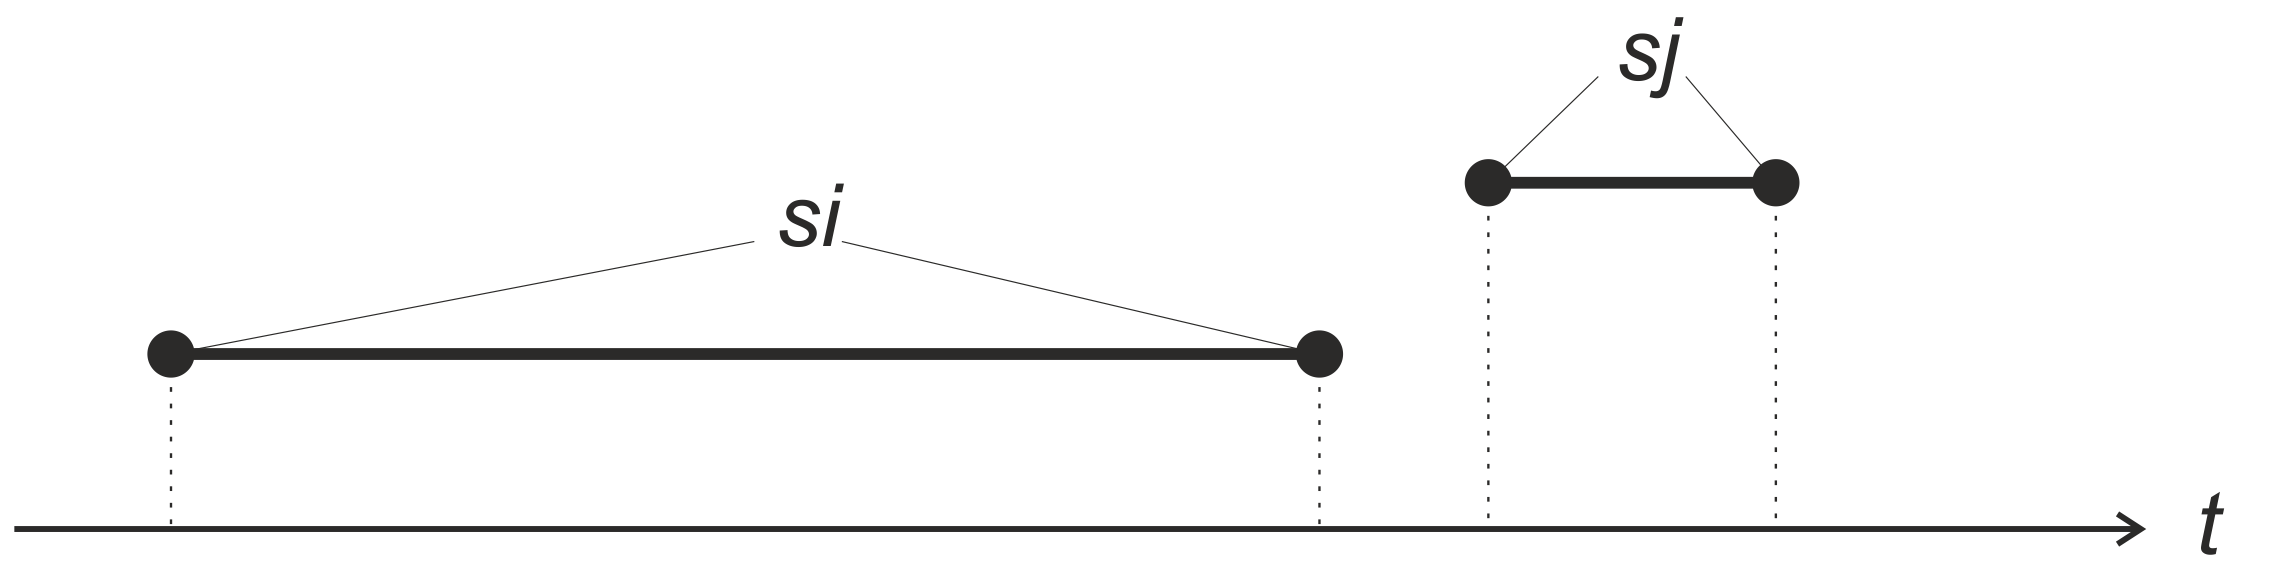
\includegraphics[scale=0.6]{./figures/sd_temp_entities/img_temporal_sequence_with_intermediate.png}
		\end{figure}
	\end{SCn}
\end{frame}

\begin{frame}{\\Темпоральные параметры}
	\topline
	\justifying
	\scnheader{параметр}
	\scnhaselement{длительность}
	\scnhaselement{начало}
	\scnhaselement{завершение}
	\scnhaselement{одновременность}
\end{frame}

\begin{frame}{\\Длительность}
	\topline
	\justifying
	\vspace{10mm}
	\begin{SCn}
		\begin{figure}[H]
			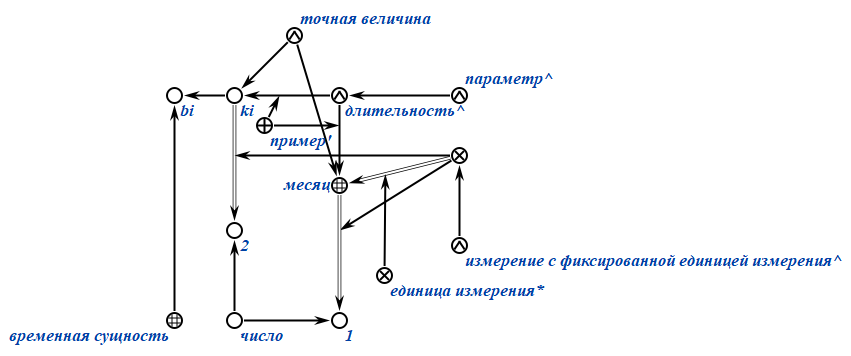
\includegraphics[scale=0.65]{./figures/sd_temp_entities/duration.png}
		\end{figure}
	\end{SCn}
\end{frame}

\begin{frame}{\\Завершение}
	\topline
	\justifying
	\vspace{10mm}
	\begin{SCn}
		\begin{figure}[H]
			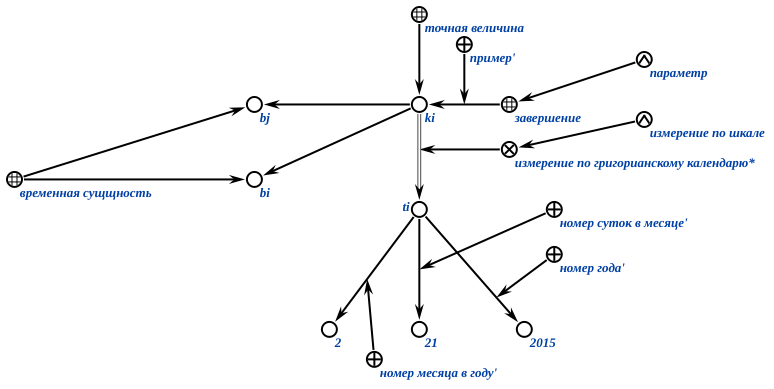
\includegraphics[scale=0.6]{./figures/sd_temp_entities/completion.png}
		\end{figure}
	\end{SCn}
\end{frame}

\begin{frame}{\\Одновременность}
	\topline
	\justifying
	\vspace{10mm}
	\begin{SCn}
		\begin{figure}[H]
			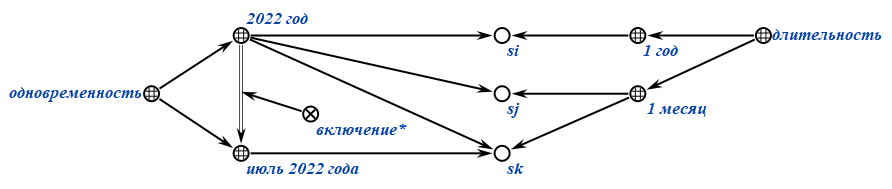
\includegraphics[scale=0.65]{./figures/sd_temp_entities/simultaneity.png}
		\end{figure}
	\end{SCn}
\end{frame}
